%! Author = tstreule
%! Date = 18.01.22

\documentclass[%
,a3paper
,fontsize=10.5pt
,landscape
,pagesize
,headinclude
]{scrartcl}
\usepackage[margin=7mm,headsep=1mm,footskip=1mm]{geometry}

% Preamble and packages
%! Author = tstreule
%! Date = 17.01.22

% Language package
% \usepackage[utf8]{inputenc} % Not to use with Xe-LaTeX!
\usepackage{fontspec}
% \usepackage{kpfonts}
% \usepackage[T1]{fontenc}
\usepackage[english,ngerman]{babel}
\usepackage[svgnames]{xcolor}

% Flush left
\usepackage[document]{ragged2e}

% Set date format
\usepackage[useregional=numeric]{datetime2}

% Arithmetic / Coding package
\usepackage{ifthen}
\usepackage{calc}

% Spacing
\usepackage[nodisplayskipstretch]{setspace}
\setlength\intextsep{0pt}% no spacing above and below figures/tables
\setlength\columnsep{10pt}% Column spacing for multicols
% \setstretch{1.1}
% Move operators tighter together
\thinmuskip=2mu                     % default: 3mu
\medmuskip=3mu plus 1mu minus 3mu   % default: 4mu plus 2mu minus 4mu
\thickmuskip=4mu plus 3mu minus 3mu % default: 5mu plus 5mu
% \setlength{\thickmuskip}{5mu}     % not possible due to \usepackage{calc}
% Array and matrix spacing
\setlength\arraycolsep{1pt}
% Hack to remove vertical spacing in equations
\usepackage{etoolbox}
\newcommand{\setdisplayskips}{%
    \setlength{\abovedisplayskip}{1pt}%
    \setlength{\belowdisplayskip}{1pt}%
    \setlength{\abovedisplayshortskip}{1pt}%
    \setlength{\belowdisplayshortskip}{1pt}}
\appto{\normalsize}{\setdisplayskips}
\appto{\small}{\setdisplayskips}
\appto{\footnotesize}{\setdisplayskips}

% Control (primitive) list items
\usepackage{enumitem}
\setlist{leftmargin=*,nosep,labelsep=2pt,parsep=-0.2pt}  % reduce spaces
\setlist[itemize,2]{label=$\circ$}

% Formatting
\usepackage{multicol, multirow, tabularx}
\usepackage{makecell}
\usepackage{ulem} % for custom underline/strikethrough/...
\usepackage{float}

% Images
\usepackage{graphicx}

% Custom emphasizing
\colorlet{emph-text-color}{MediumOrchid}
\DeclareTextFontCommand{\emph}{\color{emph-text-color}\bfseries\sffamily}


% =============
% === FONTS ===

% Font sizes
\setkomafont{section}{\normalsize}
\setkomafont{subsection}{\normalsize}
\setkomafont{subsubsection}{\normalsize}
%\setkomafont{paragraph}{\normalsize}
%\setkomafont{subparagraph}{\normalsize}

% Set fonts
\setmainfont[LetterSpace=-1.5,WordSpace=0.8,Scale=1.0,
    BoldFont=* SemiBold,BoldItalicFont=* SemiBold Italic]{Noto Serif}
\setsansfont[LetterSpace=-1.8,WordSpace=0.8,Scale=1.0]{Open Sans}

\defaultfontfeatures{Mapping=tex-text}
\defaultfontfeatures{Ligatures=TeX}
\addfontfeature{LetterSpace=-20.0}


% ====================
% === TITLE FORMAT ===

\usepackage{titling}

% Reduce default vertical space before and after
\setlength{\droptitle}{-3.5em}
\renewcommand{\maketitlehookd}{\vspace{-1.3em}}

% Title
\pretitle{\centering\sffamily\large\bfseries}
\posttitle{\par}
% Author
\preauthor{\centering\sffamily\small}
\postauthor{\ifx\thedate\empty{\par}\else{}\fi}
% Date - remove spacing above and below
\predate{\centering\sffamily\small\ifx\thedate\empty{}\else{\;-\;}\fi\itshape}
\postdate{\ifx\thedate\empty{}\else{\par}\fi}


% =======================
% === SECTIONS FORMAT ===

% Make spacing tight
\RedeclareSectionCommands[%
    runin=false,
    beforeskip=1ex plus .5ex,
    afterskip=0ex plus .1ex,
]{section,subsection,subsubsection}

% Define colors
\colorlet{section-color}{RoyalBlue!90}
\colorlet{subsection-color}{RoyalBlue!40}
\colorlet{subsubsection-color}{RoyalBlue!20}
\colorlet{section-text-color}{white}
\colorlet{subsection-text-color}{black}
\colorlet{subsubsection-text-color}{black}

% Put in colored box with fixed height
\def\sectionboxheight{.7em}
\def\sectionboxvspace{-.1ex}
\makeatletter
\renewcommand\sectionlinesformat[4]{%
    \colorbox{#1-color}{%
        \begin{minipage}[b][\sectionboxheight][t]{\dimexpr\linewidth-2\fboxsep\relax}
            \vspace{\sectionboxvspace}%
            \raggedsection\color{#1-text-color}\@hangfrom{#3}{#4}%
            \vspace{\sectionboxvspace}%
        \end{minipage}%
    }}
\makeatother


% ===========================
% === HEADERS AND FOOTERS ===

\usepackage[footsepline]{scrlayer-scrpage}

\pagestyle{plain.scrheadings}

% Clear and set styles
\clearpairofpagestyles
%\clearscrheadfoot
\setkomafont{pageheadfoot}{\color{gray}\sffamily}

% Reset pagination format
\setkomafont{pagination}{}

% Set content
%\ihead*{}
%\chead*{}
%\ohead*{tstreule $\vert$ Page \pagemark}
%\ifoot*{}
%\cfoot*{}
%\ofoot*{}


% =====================
% === COLOR STYLING ===
% \everymath\expandafter{\the\everymath\color{MediumBlue}}
% --> use "\the\everymath" for default math color
% --> use "\normalcolor" for other way around

\usepackage{../shortcuts}

% Uncomment for debugging headers
% \usepackage{showframe}

\graphicspath{{./graphics/}} % Set graphic path

% >>> [BEGIN] (Re-)formatting >>>
\let\degree\relax\usepackage{mathabx}
\usepackage{siunitx,amscd,esint,svg}
\usepackage[version=4]{mhchem}
%\let\oldhighlight\highlight
%\RenewDocumentCommand\highlight{s O{} m}{%
%	IfBooleanTF#1{\oldhighlight*{#2}{#3}}{\oldhighlight{#2}{#3}}}
% <<< [END] (Re-)formatting <<<

% Set title
\title{Biomedical Imaging}
\author{Timo Streule, tstreule@ethz.ch}
\date{\today}

% ======================
% === BEGIN DOCUMENT ===

\begin{document}

	%! Author = tstreule
%! Date = 17.01.22

\providecommand\thetitle{LECTURE\_NAME}

\begingroup
%\vspace*{\fill}
%\begin{center}
\begin{minipage}{.35\textwidth}

    \setmainfont{Noto Serif}
    \KOMAoptions{fontsize=12pt}\color{black}
    \justifying

    {\Large\bfseries Disclaimer}

    This document is an exam summary and follows the given material of the lecture {\itshape \thetitle}.
    Its contribution is a short summary that contains the most important concepts, formulas and algorithms.
    Due to curriculum content updates, some content may not be relevant to future versions of the course.

    I do not guarantee the accuracy or completeness, nor is this document endorsed by the instructors.
    Any errors that are pointed out to me are welcome.
    The complete {\LaTeX} source code can be found at {\ttfamily https://github.com/tstreule/eth-cheat-sheets}.

\end{minipage}
%\end{center}
%\vspace*{\fill}
\endgroup

\pagebreak


	\begin{multicols*}{4}

		% Suppress enumeration of sections
		%\setcounter{secnumdepth}{0}

		\maketitle

		%! Author = tstreule

\section*{General}

\subsection*{Formeln}
%
\textbf{Circle}: $U\ped{circle} = 2\pi r$, $A\ped{circle} = \pi r^2$

%	\textbf{Laplace}:\\
%	\begin{tabular}{ c@{$\;\laplace\;$}c c c@{$\;\laplace\;$}c }
%		$f(at)$			& $\frac{1}{\abs{a}}F(s/a)$	&& $f(t-a)$		& $\eu^{-as}F(s)$\\
%		$f(t)\eu^{at}$	& $F(s-a)$					&& $f'(t)$		& $sF(s) - f(0^+)$\\
%		$t^n$			& $n!/s^{n+1}$				&& $t^n f(t)$	& $(-1)^n F^{(n)}(s)$\\
%		$\sin(at)$		& $\frac{a}{s^2 + a^2}$		&& $\cos(at)$	& $\frac{s}{s^2 + a^2}$\\
%		$\eu^{at}$		& $\frac{1}{s - a}$			&& $t^n \eu^{at}$& $\frac{n!}{(s-a)^{n+1}}$
%	\end{tabular}

\textbf{Constants}:\\
\begin{tabular}{r@{$\;=\;$}l}
    $h$			& $\unit[6.626 {\scriptstyle\mathrm{E}-34}]{Js} = \unit[4.135 {\scriptstyle\mathrm{E}-15}]{eV\,s}$,
    \quad $\hbar = \frac{h}{2\pi}$,
    \quad $hc = \unit[1.986 {\scriptstyle\mathrm{E}-25}]{Jm}$\\
    $\epsilon_0$& $\unitfrac[8.85 {\scriptstyle\mathrm{E}-5}]{As}{Vm}$\\
    $\mu_0$		& $\unitfrac[4\pi {\scriptstyle\mathrm{E}-7}]{N}{A^2}$\\
    $k\ped{B}$	& $\unitfrac[1.38 {\scriptstyle\mathrm{E}-23}]{J}{K} = \unitfrac[8.617 {\scriptstyle\mathrm{E}-5}]{eV}{K}$\\
    $q$			& $\unit[1.602 {\scriptstyle\mathrm{E}-19}]{C}$, \quad $m_e = \unit[9.109 {\scriptstyle\mathrm{E}-31}]{kg}$, \quad $m_p = \unit[1.672 {\scriptstyle\mathrm{E}-27}]{kg}$\\
    $F$			& $\unitfrac[96485]{C}{mol}$ (Faraday)\\ % charge of 1 mole of electrons
    $R$         & $N\ped{A} k\ped{B} = \unitfrac[8.314]{J}{mol\;K}$ (Ideal gas constant)\\
    $N\ped{A}$	& $\unitfrac[6.022 {\scriptstyle\mathrm{E}23}]{particles}{mol}$
    \qquad $\SI{0}{\degreeCelsius} = \unit[273.15]{K}$
\end{tabular}
%%%%%%%%%%%%%%%%%%%%%%%%%%%%%%%%%%%%%%%%%%%%%%%%%%%%%%
\subsection*{Einheiten}
%
\formula{Druck}{\unit[1]{Pa} = \unitfrac[1]{N}{m^2} = \unitfrac[1]{J}{m^3} = \unitfrac[10]{g}{cm\cdot s^2}}\\
\formula{Induktivität}{\unit[1]{H} = \unitfrac[1]{Vs}{A} = \unit[1]{\Omega\,s}}\\
\formula{Power}{\unit[1]{W} = \unitfrac[1]{J}{s} = \unit[1]{VA}}\\
\formula{electron volt}{\unit[1]{eV} = \unit[1.602 {\scriptstyle\mathrm{E}-19}]{J} = \unitfrac[23.06]{kcal}{mol}}\\
\formula{Charge}{\SI{1}{\coulomb} = \SI{1}{\ampere\second}}\\
\formula{Energy}{\SI{1}{\joule} = \unitfrac[1]{kg\;m^2}{s^2} = \unit[1]{Nm} = \unit[1]{VAs} = \unit[1]{CV} = \unit[1]{Ws}}\\
%%%%%%%%%%%%%%%%%%%%%%%%%%%%%%%%%%%%%%%%%%%%%%%%%%%%%%
\subsection*{Good to know}
%
\formula{Power in \unit{dB}}{10\,\log_{10}\frac{I}{I_0}}\\
\formula[\unit{\frac{\!W}{m^2}}]{Intensity}{ I = \frac{\textrm{avg. Power }(P)}{\textrm{area }(A)} }\\
\formula[\unit{W} = \unit{\frac{kg\,m^2}{s^3}}]{avg. Power}{P = \frac{\textrm{avg. Work in cycle }(\overline{W})}{\textrm{cycle }(T)}}\\
\formula[\unit{J}=\unit{Ws}]{(avg.) Work}{\overline{W} = \int_{\textrm{cycle}} \frac{1}{\textrm{cycle} (T)} \cdot \vec{F}\cdot\vec{x} \diff t }\\

mass $m$ vibrates with an amplitude $a$ along $x$-axis:\\
$\vec{x}(t) = a\sin(\omega t)\cdot \vec{e}_x, \quad \omega = 2\pi f = 2\pi/T, \quad \vec{F}(t) = m\,\ddot{\vec{x}}(t)$
%%%%%%%%%%%%%%%%%%%%%%%%%%%%%%%%%%%%%%%%%%%%%%%%%%%%%%
\subsection*{NuS}
%
\formula{Induktivität}{u(t) = L \deriv{i_L}{t} \enskip\laplace\enskip U(s) = sL\,I_L(s)}\\
\formula{Konduktivität}{i(t) = C \deriv{u_C}{t} \enskip\laplace\enskip U(s) = \frac{1}{sC}\,U_C(s)}\\

\formula{Transformator}{u_1 = L_1 \deriv{i_1}{t} - M \deriv{i_2}{t} \textnormal{,\enskip $M$: mutual inductance}}\\
\formula{LCR-Schwingkreis}{\omega_0 = 2\pi f_0 = 1/\sqrt{LC}}\\
%%%%%%%%%%%%%%%%%%%%%%%%%%%%%%%%%%%%%%%%%%%%%%%%%%%%%%
\subsection*{Laplace}
%	%Laplace Transformation: \;
%	$\phantom{\laplace} \dis{0.4} u(t)=\mathcal{L}^{-1}\{U(s)\} = \frac{1}{2\pi\iu} \int_{\bar{s}}^s U(s)\eu^{st} \diff s$\\
%	$\laplace \dis{0.4} U(s)=\mathcal{L}\{u(t)\} = \int_0^\infty u(t)\eu^{-st} \diff t$
%
\begin{tabular}{ rcl }
    \toprule
%		$u(t)$							& \laplace	& $U(s)$								\\%\addlinespace
%		\midrule
    $\lambda\;u(t) + \mu\;v(t)$		& \laplace	& $\lambda\;U(s) + \mu\;V(s)$			\\
    ${u(at),\; \scriptstyle a>0}$	& \laplace	& $\frac{1}{a}$ $U(\frac{s}{a})$		\\
    { \color{red} $u(t-t_0)$ }		& \laplace	& $\eu^{-st_0}$ $U(s)$					\\
    $\eu^{-at}$ $u(t)$				& \laplace	& { \color{red} $U(s+a)$ }				\\
    ${ (-t)^{n} u(t) }$				& \laplace	& $U^{(n)}(s)$							\\
    $u^{(n)}(t)$					& \laplace	& $ {s^nU(s) - \ldots - u^{(n-1)}(0)} $	\\
    \midrule
%		$t^n$							& \laplace	& $\frac{n!}{s^{n+1}}$					\\\addlinespace
%		$\eu^{-at}$						& \laplace	& $\frac{1}{s+a}$						\\\addlinespace
%		$t\eu^{-at}$					& \laplace	& $\frac{1}{(s+a)^2}$					\\\addlinespace
%		$t^n\eu^{-at}$					& \laplace	& $\frac{n!}{(s+a)^{n+1}}$				\\\addlinespace
%		$\sin (at)$						& \laplace	& $\frac{a}{s^2+a^2}$					\\\addlinespace
%		$\cos(at)$						& \laplace	& $\frac{s}{s^2+a^2}$					\\\addlinespace
    \multicolumn{3}{c}{
        \begin{minipage}{.45\columnwidth} \centering
        \begin{tabular}{ ccc }
%					$u(t)$							& \laplace	& $U(s)$								\\%\addlinespace
%					\midrule
            $t^n$							& \laplace	& $\frac{n!}{s^{n+1}}$					\\
            $\eu^{-at}$						& \laplace	& $\frac{1}{s+a}$						\\
            $t\eu^{-at}$					& \laplace	& $\frac{1}{(s+a)^2}$					\\
        \end{tabular}
        \end{minipage}%
        \begin{minipage}{.45\columnwidth} \centering
        \begin{tabular}{ ccc }
%					$u(t)$							& \laplace	& $U(s)$								\\%\addlinespace
%					\midrule
            $t^n\eu^{-at}$					& \laplace	& $\frac{n!}{(s+a)^{n+1}}$				\\
            $\sin (at)$						& \laplace	& $\frac{a}{s^2+a^2}$					\\
            $\cos(at)$						& \laplace	& $\frac{s}{s^2+a^2}$					\\
        \end{tabular}
        \end{minipage}
    }\\
    \bottomrule
\end{tabular}

		%! Author = tstreule

\section{Generation of X-rays}

\subsection{Basic formulas}
%
\begin{itemize}
    \item \highlight{$\displaystyle c = \frac{1}{\sqrt{\mu_0\epsilon_0}} = \lambda\nu$}
    \highlight{$\displaystyle E = h\nu = \frac{hc}{\lambda}$}
    \hfill rest mass: $mc^2=\unit[511]{eV}$
    \item Range of X-Rays: $\lambda = \unit[10]{pm} - \unit[10]{nm}$
    \item $E\ped{radiation} = n \cdot E\ped{photon}$ \quad with \quad $E\ped{photon} = h \cdot \nu = e U_a$
    \item $p\ped{photon} = mc = h/\lambda, \qquad \lambda\ped{min} = \frac{hc}{e U_a}$
\end{itemize}
%%%%%%%%%%%%%%%%%%%%%%%%%%%%%%%%%%%%%%%%%%%%%%%%%%%%%%
\subsection{Spectrum}
%
Photon flux vs E: Speaks by \textbf{Characteristic Radiation}.

Continuous spectrum by \textbf{Bremsstrahlung}: 1st el. deflection: Spectrum $0-E_{max}$, 2nd el. defl. Not to $E\ped{max}$ anymore.

If material changes: $E\ped{max} = const$, slope changes\\
If E changes: slope const., intersection with E-axis @ E

Low-Energy rad. absorbed anyway $\to$ Al filter $\to$ dose $\downarrow$
%%%%%%%%%%%%%%%%%%%%%%%%%%%%%%%%%%%%%%%%%%%%%%%%%%%%%%
\subsection{Heat generation \& dissipation}
%
Efficiency: $\eta = \frac{\textrm{absorbed power}}{\textrm{incident power}} = 1\%$\\
$P_\textrm{heat} = U_a \cdot I_a \cdot (1-\eta)$ \textcolor{gray}{$= P - P_\textrm{X-ray}$}

\textbf{Dissipation} (Infrared): Diffusion ($\propto T^4$) and\\
Radiation ($\propto\Delta T$): $\lambda$ vs. $I$, $\lambda_\textrm{peak} = b/T$, $b = \unit[2.9\E{-3}]{mK}$

		%! Author = tstreule

\section{Imaging with X-rays}

In $\log E$ vs. $\log\mu$ plot is Compton linear, but Photo decreasing.
\begin{itemize}
    \item \textbf{Photo effect, char. radiation} (Desired):
    Photon gets completely absorbed by throwing an electron out of atom $\to$ damage.
    \textbf{Probability} $\propto \rho\cdot Z^3/E^3$,
    \textcolor{gray}{$\rho$: tissue density}\\
    \textit{Effective in} contrast agent, lead, bone
    \item \textbf{Compton Scattering} ($\to$ resolution loss):
    Photon only gets deflected.
    \textbf{Probability:} $\propto \rho/E$\\
    \textit{Effective in} water, air, soft tissue, bone\\
    Scattering angle $\phi$: \highlight{$\displaystyle \lambda_p - \lambda_{p'} = \frac{h}{m_c \cdot c} (1 - \cos \phi)$}
\end{itemize}
To only have photo effect $\to$ $E\downarrow$. Compromise with thick targets.

\textbf{Spatial resolution}: MTF is indicated in const vs \textbf{l}ine \textbf{p}airs/mm

\textbf{Temporal resolution}: periodic s.t. $\Delta t<1/\textrm{BW}\ped{heartbeat}$
%%%%%%%%%%%%%%%%%%%%%%%%%%%%%%%%%%%%%%%%%%%%%%%%%%%%%%
\subsection{Attenuation coefficients \hfill\textnormal{efficient for small $E$}}
%
\textbf{Mass absorption}: $\mu' = \frac{A\ped{eff}N\ped{A}}{\textrm{atomic weight}} [\unitfrac{cm^2}{g}]$ \hfill area to collide with\\
\textbf{Linear attenuation}: $\mu = \mu' \cdot \rho [\unit{cm^{-1}}]$

\textbf{Beer-Lambert's law}: $I = \int \limits_0^{E\ped{max}} I_0(E) \eu^{-\int_{-\infty}^{\infty} \mu(E,x)\diff x}\diff E$\\
$\mu$ homog.: \highlight{$\displaystyle I = I_0 \eu^{-\mu x}$} \hfill \textbf{Contrast} $\propto (\mu_1 - \mu_0)d = \ln(I_0/I)$
%%%%%%%%%%%%%%%%%%%%%%%%%%%%%%%%%%%%%%%%%%%%%%%%%%%%%%
\subsection{Detector Technology}
%
Analog photographic film: $Ag^+ + Br^- \underbrace{\longrightarrow}_{photon} AgBr$\\
Use fluorescent screen (spacial res.$\uparrow$) $\longrightarrow$ 5x efficiency

\textbf{Anti-scatter grid}:
No grid: $c\ped{scatter} = \frac{(I+I_S) - (I_B + I_S)}{I_B + I_S} = c \cdot \frac{1}{1 + I_S/I_B}$ where $c = \frac{I - I_B}{I_B}$ is contrast with grid

\textbf{Digital Detector}: photofilm, excited el's $\to$ laser $\to$ PMT

\textbf{DSA}: Contrast Agent: Iodine: increases x-ray absorption.

		%! Author = tstreule

\section{Computed Tomography}

Quantitative with \textbf{Houndsfield unit} (normed to water):\\
\highlight{$\displaystyle \textrm{CT value} = \frac{\mu - \mu\ped{water}}{\mu\ped{water}}\cdot \unit[1000]{HU}$}

Beam types: Pencil, Fan, Parallel fan, cone.

\textbf{Algebraic Reconstruction}:
Out of a $n \times n$-Image, make a $n^2 \times n^2$ equation system:
$\vec{P} = W \vec{\mu}$ (P are the measurements, W are the weightings, how much a beam crossed a box/pixel)\\
\highlight{$\displaystyle \vec{\mu} = (W^H W)^{-1} W^H \vec{P}$} $~^H$: hermetisch transponiert.

\textbf{Projection Slice Theorem}: Project a 2D function onto a line and do a 1D Fourier transform \quad $\iff$\\
Do a 2D Fourier transform of that 2D function and slice it through its origin (parallel to the line above).
%%%%%%%%%%%%%%%%%%%%%%%%%%%%%%%%%%%%%%%%%%%%%%%%%%%%%%
\subsection{Backprojection}
%
When doing simple Backprojection: $PSF = \frac{1}{|r|}$

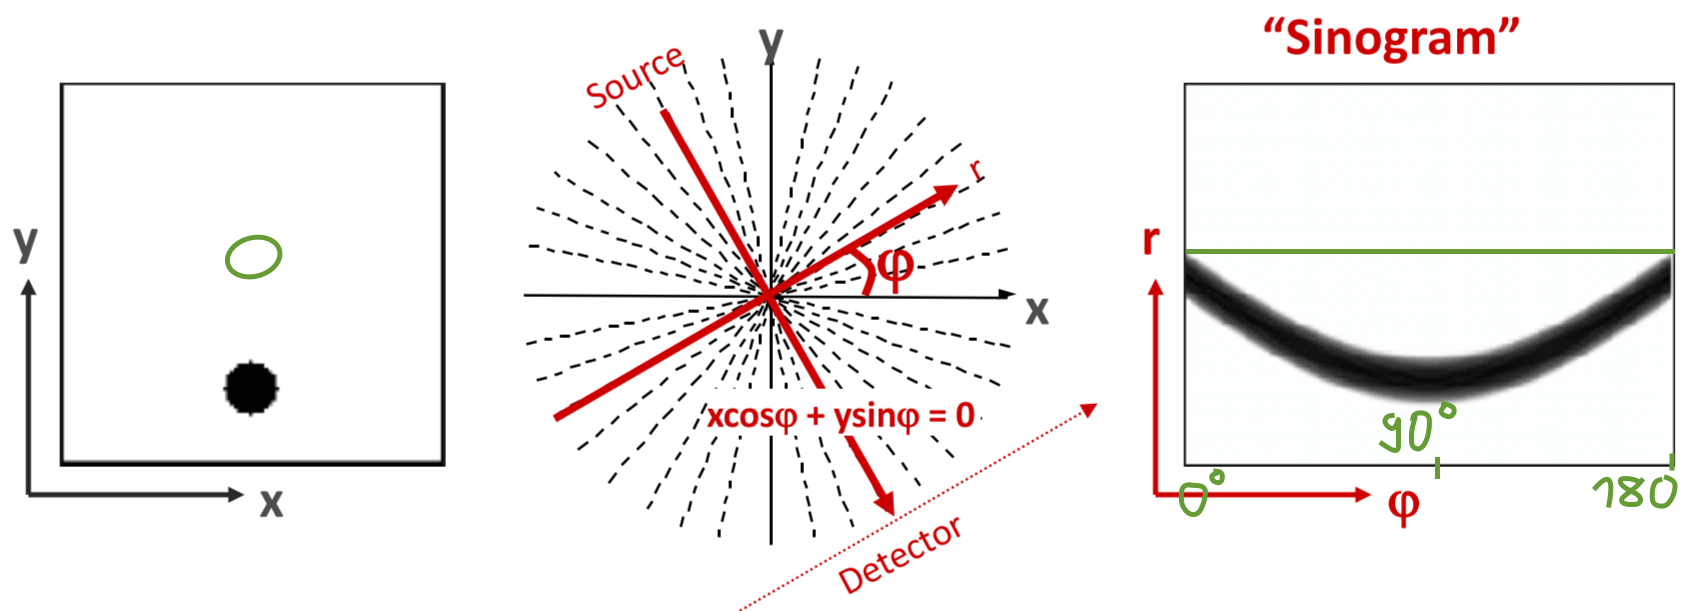
\includegraphics[width = .8\linewidth]{CT_Sinogram}\\
$P_\phi(r) = -R[\mu](r, \phi) = -\iint \limits_{-\infty}^\infty \mu(x, y) \delta(\underbrace{x \cos \phi + y \sin \phi - r\vspace{-1mm}}_{\text{line formula}\vspace{-1mm}})dxdy$

Math. Deduction: \textbf{1st Reconstruction formula}:\\
Projection $P_\phi(r) = -\int \mu(r, s) ds$\\
$\mathcal{F}\{P_\phi(r)\}(u,\phi) = \int P_\phi(r) e^{-jur}dr =$\\
$= - \iint \mu(r, s) e^{-jur} dr ds =$ (with $r = x\cos \phi + y \sin \phi$)\\
$= -\iint \mu(x, y) \exp(-jx\underbrace{u \cos \phi\vspace{-1mm}}_{\vspace{-2mm}p \hat{=} k_x} - jy\underbrace{u\sin\phi\vspace{-1mm}}_{\vspace{-2mm}q \hat{=} k_y}) dxdy = $\\
$= - \iint \mu(x, y) e^{-jxp - jyq} dx dy$ (until here just proj. slice th.)\\
\highlight{$\displaystyle \implies \mu(x, y) = \frac{-1}{4\pi^2}\iint \mathcal{F}\{P_\phi(r)\}(p, q) \eu^{\iu xp + \iu yq} \diff p\diff q$}\\
Fill k-space with $\mathcal{F}$ of the proj.s $\hat{=}$ Backproj. of $\mathcal{F}$\\
Then do 2D-backtransformation

\textbf{2nd variant}: Change of integration variables:\\
\fbox{$u(x,y) = \frac{-1}{4\pi^2} \int \limits_0^\pi \int \limits_{-\infty}^\infty \mathcal{F}\{P_\phi(u)\}\eu^{\iu ur} \abs{u} \diff u \diff\phi$}

\textbf{Filtered Backprojection}:\\
$\highlight{\hat{u}(x, y) = \int_0^\pi P_\phi \cdot \mathcal{F}^{-1} \{|u|\} d\phi} = \sum_{j=0}^n \big( p(r,\varphi_j)*h(r) \big) \textrm{d}\varphi$.
%%%%%%%%%%%%%%%%%%%%%%%%%%%%%%%%%%%%%%%%%%%%%%%%%%%%%%
\subsection{Effects that occur in practice \& Spiral CT}
``Streak artifacts'': Too few projections have been acquired. Correction: Additional low-pass $\implies$ SNR rises.

``data grabbing'': Convert cartesian $\leftrightarrow$ polar coordinaates

Filter in image-domain: $|u| \quad \laplace \quad \frac{1}{(2\pi r)^2}$\\
If Fourier-domain is band-limited, the filter becomes a \textbf{Ram-Lak}: $\mathrm{sinc}(r) * \frac{1}{(2\pi r)^2}$
\quad\textcolor{gray}{(don't forget: $\mathrm{rect}(r) \quad\laplace\quad \mathrm{sinc}(r)$)}

Have other filter, in order to not amplify noise: \textbf{Shepp-Logan, Cosine or Hann-Filter}, i.e. combine with low-pass.

\textbf{Spiral CT}: Before backprojection, do linear interpolation of data. \textbf{Pitch}=1: The neighboring slices touch, Pitch=2: slice distance = 1 slice thickness
%%%%%%%%%%%%%%%%%%%%%%%%%%%%%%%%%%%%%%%%%%%%%%%%%%%%%%
\subsection{(Quantum) Noise}
%
Distribution of photon counts is $P_\lambda(x)$.
$\textrm{E}\{P_\lambda\} = \lambda \equiv \bar{N}$, $\sigma = \sqrt{\lambda}$.\\
$\!\implies \textrm{SNR} = \frac{\textrm{average}}{\textrm{std. deviation}} \!=\! \frac{\overline{N}}{\sqrt{\overline{N}}} = \sqrt{N}$\\
\phantom{$\!\implies$} where $N$: \#X-rays, $\lambda$: \#Photons registered.\\
$\!\implies \textrm{Image SNR} = \frac{\overline{I}}{\sqrt{\textrm{Var}\{I\}}}$ where $\sigma_I \equiv \sqrt{\textrm{Var}\{I\}} \propto \sqrt{\frac{1}{I_\textrm{A}\,t\,\Delta z}}$

Pixel noise = $\sigma = \sqrt{\frac{1}{M-1}\sum_{i=1}^M (I_i - \overline{I})^2} = \highlight{\sqrt{1 / (Q \Delta z) }}$\\
where Q: Tube current $I_\textrm{A}$ $\times$ scan time $t$, \quad $\Delta z$: detector thickness
%%%%%%%%%%%%%%%%%%%%%%%%%%%%%%%%%%%%%%%%%%%%%%%%%%%%%%
\subsection{Dose considerations}
%
\textbf{Absorbed dose}: $\unit[1]{Gray} = \unit[1]{Gy} = \unitfrac[1]{J}{Kg}$\\
\textbf{Equivalent dose}: $1 \unit{Sievert} = \unit[1]{Sv} = Q \cdot N \unit{Gy}$\\
with the \textbf{Quality factor Q} (mostly 1) and the \\\textbf{Pertinent factor N} (bone, lung, stomach: 0.12 - skin: 0.1)

\textbf{Excess Relative Risk}:\\
$RR = \frac{\text{Cancer Deaths/y}}{\text{Cancer Deaths control pop./y}}
\hfill\highlight{ERR = \frac{RR-1}{\text{Additional dose}}}$

It is higher for women and children. $2.5/\unit{Sv} - 0.25/\unit{Sv}$

		%! Author = tstreule

\section{SPECT \textnormal{-- Single Photon Emission CT}}

$\textrm{SNR} \propto \sqrt{\textrm{total \#detected gamma-rays}}$
%%%%%%%%%%%%%%%%%%%%%%%%%%%%%%%%%%%%%%%%%%%%%%%%%%%%%%
\subsection{Radioactivity in the body}
%
\highlight{$Q = -\frac{dN}{dt} = \lambda \cdot N \implies N(t) = N_0 \eu^{-\lambda t}$}\\
$[Q] = \unit{Curie} = \unit{Ci} = 3.7 \cdot 10^{10} \unit{Bq}$
\quad where \quad $1\unit{Bq} = 1\unitfrac{disintegration}{s}$

\textbf{Physical} $t\ped{1/2} = \frac{\ln 2}{\lambda}$, \quad \textbf{biological} $t\ped{1/2 bio} = \frac{\ln 2}{\lambda\ped{bio}}$

$N(t) = N_0 \eu^{-(\lambda + \lambda\ped{bio}) t} = N_0\eu^{-\lambda\ped{1/2 eff}t}$
\quad where \quad $t\ped{1/2 eff} = \frac{t\ped{1/2} \cdot t\ped{1/2 bio}}{t\ped{1/2} + t\ped{1/2 bio}}$

\textbf{$\gamma$ photons: Absorption} or \textbf{Scattering}: Change of direction by $\theta$. \highlight{$E_{\gamma}' = \frac{m_e \cdot c^2}{m_e c^2 / E_\gamma + 1 - \cos \theta}$}
%%%%%%%%%%%%%%%%%%%%%%%%%%%%%%%%%%%%%%%%%%%%%%%%%%%%%%
\subsection{Interaction of $\gamma$ photons with matter}
%
\textbf{Absorption} leads to ejection of orbital electron\\
\textbf{Scattering}: Change of direction by $\theta$. \highlight{$\displaystyle E_{\gamma}' = \frac{m_e \cdot c^2}{m_e c^2 / E_\gamma + 1 - \cos \theta}$}
%%%%%%%%%%%%%%%%%%%%%%%%%%%%%%%%%%%%%%%%%%%%%%%%%%%%%%
\subsection{Anger Camera}
\textbf{Collimation} necessary $\implies$ losses of 99.9\%

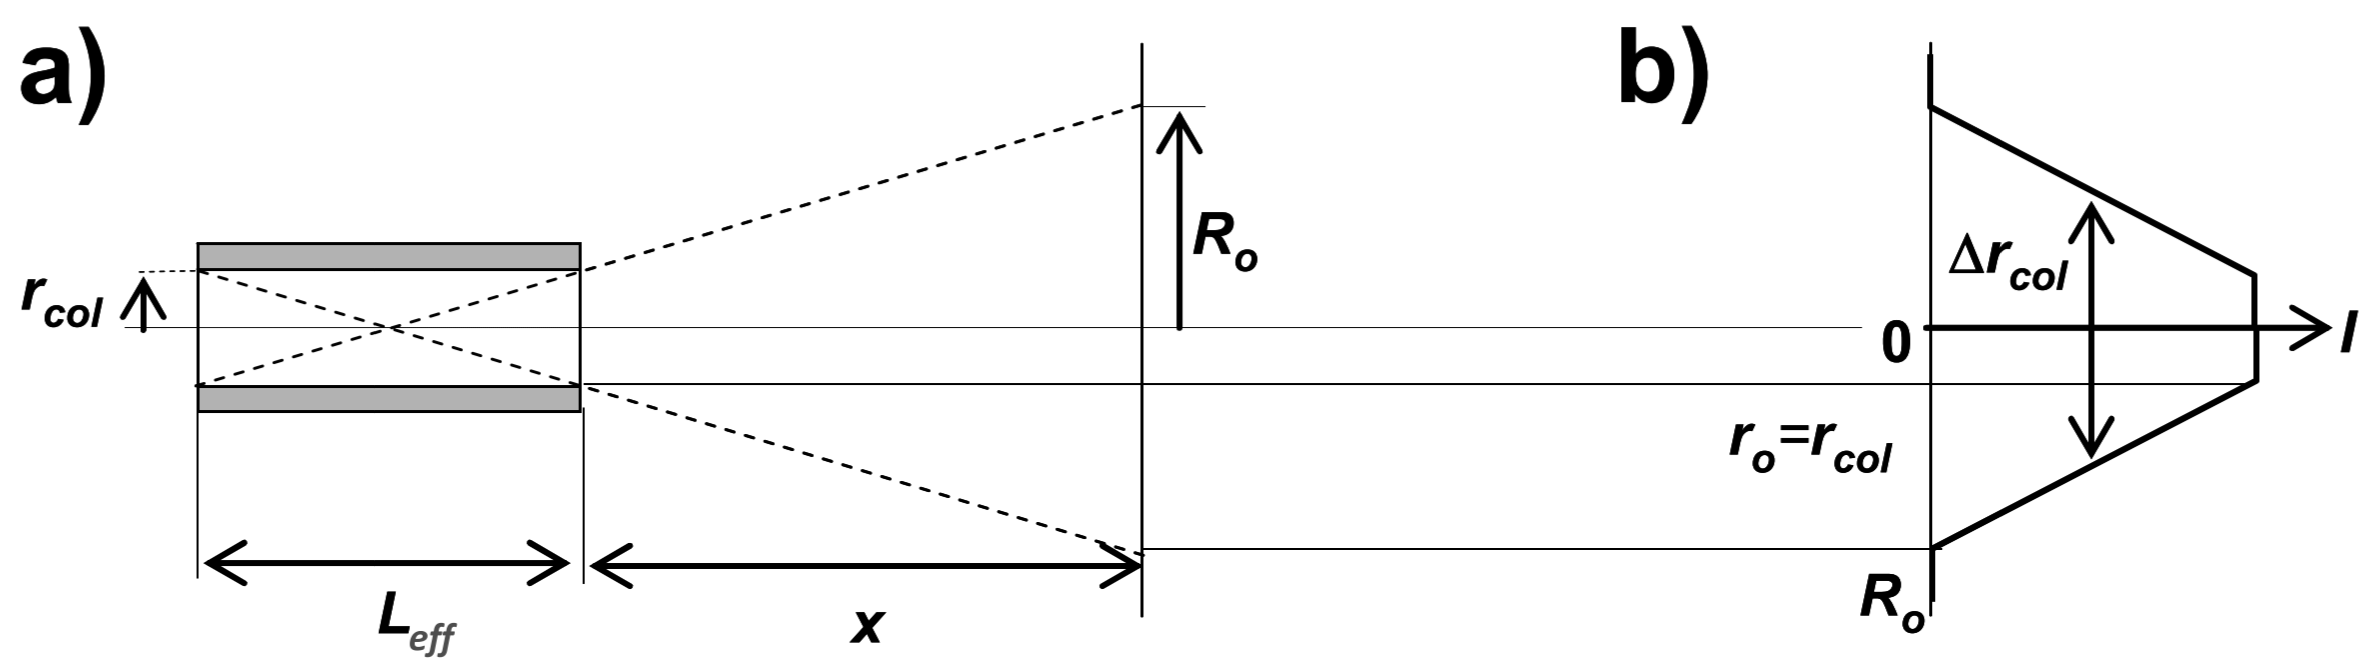
\includegraphics[width = \linewidth]{SPECT_NuclearCollimator}
Bad isolation of \textbf{septa} (lamellae) $\implies L\ped{eff} = L - \frac{2}{\mu\ped{septa}}$\\
%
\highlight{$\displaystyle R_0(x) = \frac{2 r_{col}}{L_{\text{eff}}}(x + \frac{L_{\text{eff}}}{2})$} \; \highlight{$\displaystyle \textrm{FWHM} = \Delta r_{col}(x) = \frac{2 r_{col}}{L_{\text{eff}}}(x + L_{\text{eff}})$}\\

\textbf{Signal Path}: $\gamma$-rays @140keV $\to$ Scintillation crystal $\to$ PMT $\to$ (Pos. network || pulse height analyzer) $\to$ digitizer
\begin{itemize}
    \item Scintillation crystal efficiency: \highlight{$\displaystyle \epsilon = 1 - \eu^{-\mu d}$}. $\mu$: attenuation coefficient of crystal, $d$: its thickness

    \item Usually many PMTs per crystal. Positioning network calculates where the event in the crystal was.

    \item $U_{PMT} \propto \gamma$ energy. Scattering $\implies$ $E\ped{scattered photons}\downarrow$. Pulse height analyzer has energy window $\Delta E$ around $E_0$.

    \item Poisson distributed $P_n(N)\vert \sigma^2 = \mu \implies \highlight{SNR = \sqrt{\mu}}$

    \item \textbf{Spatial resolution}: $R_{system}^2 = R\ped{gamma}^2 + R_{coll}^2$ \quad $R\ped{gamma}$ = uncertainty of positioning network. $R\ped{coll}$ see above.
\end{itemize}

\textbf{CT Version}: Res.: best at edge, worst in center. $\approx$ 7mm\\

For small objects: Use \textbf{pinhole} (cone-shaped, tungsten) camera: Problem: more dose needed, ``transparency'' around hole
%%%%%%%%%%%%%%%%%%%%%%%%%%%%%%%%%%%%%%%%%%%%%%%%%%%%%%
\subsection{Generation of Technetium}
No cyclotron needed, only generator: Essentially \ce{^{99}_{42}Mo} ($\unit[67]{h} \;\widehat{=}\; \unit[2.9\E{-6}]{s^{-1}}$) decays into \ce{^{99}_{43}Tc} ($\unit[6]{h} \;\widehat{=}\; \unit[3.1\E{-5}]{s^{-1}}$)

\textbf{Kinetic equations}:\\
$\deriv{~}{t}N_{Mo} = -k_{Mo}N_{Mo}$ and $\deriv{~}{t}N_{Tc} = k_{Mo}N_{Mo} - k_{Tc} N_{Tc}$\\
\highlight{$\displaystyle \implies N_{Tc}(t) = N_{Mo}(0) \frac{k_{Mo}}{k_{Tc} - k_{Mo}} (e^{-k_{Mo}t} - e^{-k_{Tc} t})$} {\scriptsize exp. decay}

		%! Author = tstreule

\section{PET \textnormal{-- Positron Emission Tomography}}

\begin{minipage}{.2\linewidth}
    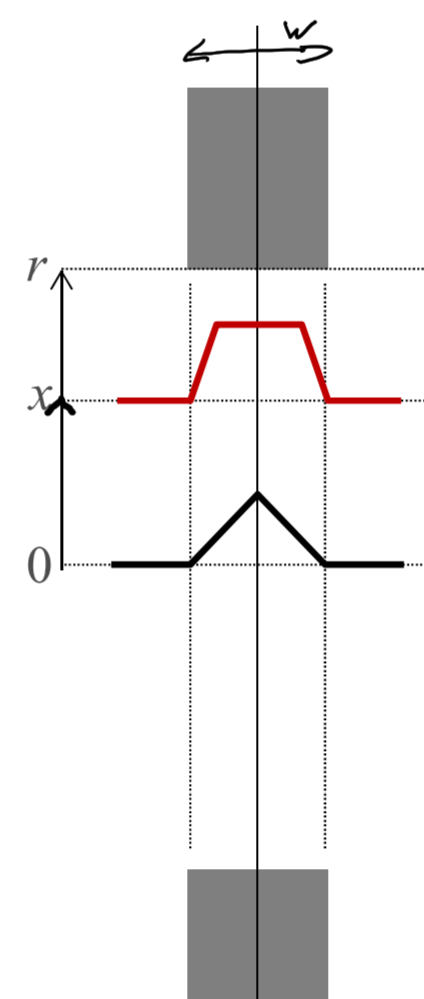
\includegraphics[width=.9\linewidth]{PET_PSF}
\end{minipage}
\begin{minipage}{.8\linewidth}
    \textbf{Positron range} $\propto$ E. \quad $\textrm{FWHM}\approx 0.1 - 0.5 \unit{mm}$.

    \textbf{Radionuclide}: $\ce{^{18}F}$ better than $\ce{^{11}C}$ (110 vs 20 min)

    \textbf{Image production}: Scintillator (fine grid) $\to$ PMT / avalance Diode $\to$ Electronics. Event finding in scintillator is linear.
    \fbox{$y = \frac{ S\ped{A}+S\ped{B}-S\ped{C}-S\ped{D} }{ S\ped{A}+S\ped{B}+S\ped{C}+S\ped{D} }$}

    \textbf{PSF}: Trapezoid/Triangle. \highlight{$\displaystyle \textrm{FWHM} = w\frac{r+x}{2r}$}\\
    {\scriptsize r: Ring diameter, x: distance from center, w: grid spacing of sc.}
\end{minipage}
%%%%%%%%%%%%%%%%%%%%%%%%%%%%%%%%%%%%%%%%%%%%%%%%%%%%%%
\subsection{Efficiency (to actually measure concentrations)}
Detection eff. $\epsilon = (1-e^{-\mu d}) \cdot \Phi$ \hfill ($\Phi$: frac. of events in E window)

Geometric eff.: $\Omega = 4\pi \sin(\arctan(z/D))$ \hfill $D=2r$, $z$: length

Radial geometric coverage $\phi$: Fraction not gap between crystals

\textbf{Total sensitivity}: \highlight{$\displaystyle \eta = \epsilon^2 \phi \frac{\Omega}{4\pi}$}
%%%%%%%%%%%%%%%%%%%%%%%%%%%%%%%%%%%%%%%%%%%%%%%%%%%%%%
\subsection{Problems, solutions and additions}
\textbf{Correction table} for which scintillator under PMT

\textbf{Correction matrix}: against non-uniform detector eff.

\textbf{Attenuation correction}: Measure Image in HU via X-Ray CT, $\to$ attenuation coeff. $\to$ multiply PET lines by $\eu^{\mu D_{ij}}$

\textbf{Random coincidence}: Measure Background noise, then -

\textbf{Detector dead time} $\delta$: $N\ped{measured} = N\ped{true} \eu^{-N\ped{true} \delta}$

\textbf{TOF} (Time Of Flight of photon): $\Delta x = \frac{c\Delta t}{2} = \unit[75]{mm} \;\widehat{=}\; \unit[500]{ps}$

\textbf{3D image reconstr.}: Use coinc. between different rings.
%%%%%%%%%%%%%%%%%%%%%%%%%%%%%%%%%%%%%%%%%%%%%%%%%%%%%%
\subsection{Quantitative PET - various effects and definitions}
\textbf{Partial voluming}: When measuring the \underline{intensity} of an object, it appears smaller at the edge of the object than it is. $\to$ Only measure in the center

\textbf{Injected dose per gram of tissue} \fbox{$\%ID/g = \frac{c_t v_t}{D_{inj}} \cdot \frac{1}{m_t} \cdot 100\%$}, \quad
$c_t$: tissue conc., $v_t$: vol. of tissue ROI, $m_t$: mass of tissue ROI, $D\ped{inj}$: injected dose

\textbf{Standardized uptake value} ($M$: Body mass, $S$: surface)\\
\highlight{$\displaystyle SUV = [\%ID/g] \cdot M/100$} \highlight{$\displaystyle SUV' = [\%ID/g] \cdot S / 100$}

\textbf{Distribution volume}: Volume of blood needed for $M$ \#tracer.\\
\fbox{$V_d = M/c_b = V_t c_t/c_b + V_b = V_t \lambda + V_b$} \quad $\lambda =  c_t/c_b$\\
$V_t \lambda = V_1$ = equiv blood vol. to tissue vol. where tracer is\\
$c_b$: typ. conc. of that tracer in blood. $V_d > 7 \ell \implies$ body.
%%%%%%%%%%%%%%%%%%%%%%%%%%%%%%%%%%%%%%%%%%%%%%%%%%%%%%
\subsection{The scatchard equation}
\textbf{\underline{L}igand} (tracer/drug), \textbf{\underline{R}eceptor}. \quad Reaction: L+R = RL

$[L], [R], [RL]$: conc. ---
$[R_T]$: total \#receptors ---
$k\ped{off}, k\ped{on}$: reaction rates ---
$k\ped{off} \cdot [RL]$: \#bound pairs that separate.

Equilibrium eq.: $k\ped{off} \cdot [RL] = k\ped{on} \cdot [R] \cdot [L]$ \\
Eq. const.: $K_d = \frac{k\ped{off}}{k\ped{on}} = \frac{[R] \cdot [L]}{[RL]}$ \hfill
\highlight{$\displaystyle \frac{[RL]}{[L]} = -\frac{1}{K_d} \cdot [RL] + \frac{R_T}{K_d}$}\\
Scatchard plot: $\textrm{slope} = 1/K_d$, $R_T$: intersection with $[RL]$-axis
%%%%%%%%%%%%%%%%%%%%%%%%%%%%%%%%%%%%%%%%%%%%%%%%%%%%%%
\subsection{Kinetic models}
\textbf{Renking-Crone eq.}: (amount of substance diffuses out of a blood capillary)\\
\highlight{$\displaystyle = F \cdot E$} \highlight{$\displaystyle E = 1 - \eu^{-P \cdot S / F}$}
$E$: Efficiency, $P$: vascular permeability, $S$: capillary surface, $F$: blood flow

\textbf{Kinetic model}: ($c_p$: Plasma $\leftarrow$ particular part)\\
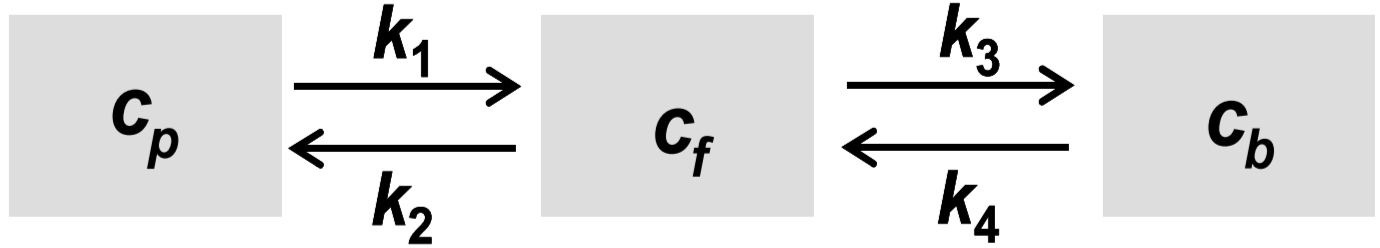
\includegraphics[width = 0.45\linewidth]{PET_Kinetic_Model}
$c_f$: free ligands, $c_b$: bound l

\textbf{Kin. eq.}:
$\deriv{c_f}{t} = k_1 c_p - (k_2 + k_3) c_f + k_4 c_b$, \;---\;
$\deriv{c_b}{t} = k_3c_f - k_4c_b$, \;---\;
$k_1 = FE$, \;---\;
$k_2 = k_1 c_p/c_f$, \;---\;
$k_3 = k_{on} [R]$, \;---\;
$k_4 = k_{off}$

What is measured: $c_t(t) = c_f(t) + c_b(t)$. $* c_p(t)$ should be in the equation. $\to$ At the end determine the rate constants.

\textbf{Improvement}: Look at reference section in brain without receptors. Only 2 compartment model, measure $k_1$ and $k_2$.

To measure behaviour of a drug (cold): Tracer (hot) $\to$ same receptors. Experiment with and without drug. Assumption: $c_b << c_{b,d}$. The drug changes the \# total receptors from $B_{max}$ to $B'_{max}$. \textbf{Receptor occupancy for drug}:\\
\fbox{$\textrm{RO}[\%] = \frac{c_{b,d}}{B\ped{max}} = (1 - B'\ped{max}/B\ped{max})\cdot 100\%$}

		%! Author = tstreule

\section{MRI}

\subsection{Quantum basics}
\textbf{Spin} $S_z = \hbar m \quad m = -I, -I+1, ... I \quad |S| = \hbar \sqrt{I(I+1)}$\\
\textbf{Magnetic moment}: \fbox{$\vec{\mu} = \gamma \vec{S}$} ($\gamma$: gyromagnetic ratio)\\
\textbf{Energy content} in $\vec{B}$-Filed: \fbox{$E_m = -\vec{\mu} \cdot \vec{B} = \pm \frac{\hbar}{2} \gamma B_0$}\\
\textbf{Blotzmann stat.}: $\frac{n\ped{-1/2}}{n\ped{+1/2}} = \exp(-\frac{\Delta E_m}{k\ped{B} T})$ \quad $\frac{\Delta n}{n} \propto \frac{\gamma \hbar B_0}{2 k\ped{B} T}$\\
\textbf{Larmor frequency}: E gap $\leftrightarrow$ photons: \highlight{$\displaystyle \omega_L = \gamma B_0$}\\
\textbf{Macrosc. mag. dipolar moment}: \fbox{$\vec{M}_0 = \sum \vec{\mu} = \Delta n \mu_z$}

\textbf{Bloch equation} ($T_2 << T_1$)\\
\highlight{$\displaystyle \frac{d}{dt}\vec{M} = \left( \begin{matrix}
                                        -1/T_2 & -\gamma B_z & \gamma B_y \\
                                        \gamma B_z & -1/T_2 & -\gamma B_x \\
                                        -\gamma B_y & \gamma B_x & -1/T_1\end{matrix} \right) \vec{M} + \left( \begin{matrix}
                                                                                                                   0 \\ 0 \\ M_0 / T_1 \end{matrix} \right)$}\\
{\small $M_z(t) = M_0\cos\alpha + (M_0-M_0\cos\alpha) (1-\exp(-t/T_1))$, \hfill $\alpha = \gamma B_1\tau\ped{B1}$: tip angle}

$\vec{B}$ with $|\vec{B}| = B_1 = const$ and $B_z = B_0$ spinning with $\omega_{RF}$ around the z-Axis. $\omega_{RF} = \omega_L \iff \vec{M}$ spins $\downarrow, \uparrow, \downarrow$ etc.

\textbf{Rot. frame of reference}: $\vec{B}$ stays at a slight angle and $\vec{M}$ rotates around it. Correction: $B_z = B_0 - \omega_{RF} / \gamma$
%%%%%%%%%%%%%%%%%%%%%%%%%%%%%%%%%%%%%%%%%%%%%%%%%%%%%%
\subsection{Basic setup}
\begin{minipage}{\linewidth}
    \begin{enumerate}
        \item Have $B_z$ + rot. field to push spins in x-y-plane.
        \item Coils to make gradients: Maxwell (z), and two Golay pairs
        \item Changing the gradient $\to$ travel k-space and sample it
        \item IFFT to get the image weighted with proton density
    \end{enumerate}
\end{minipage}

Signal from entire obj: \qquad $S(t) = \eu^{\iu \omega_0 t} \int\ped{obj} \rho(\vec{r})\eu^{\iu \vec{k} (t) \cdot \vec{r}} \diff^3 \vec{r}$\\
Fourier transform of $\rho(\vec{r})$: \quad $S(\vec{k}) = \eu^{-\iu \omega_0 t} \int\ped{obj} \rho(\vec{r})\eu^{-\iu \vec{k} \cdot \vec{r}} \diff^3 \vec{r}$

\textbf{Slice sel.}: Grad. in z-dir. and flip spins with a sinc$\times$gauss-pulse ($\approx \laplace$ rect, range of freq. where $\Delta B_z = 0$).

Grad. $\to$ \textbf{dephasing}. $\implies$ invert G to \textbf{rephase} spins.

\subsubsection{Measuring the spin}
\fbox{$\hat{U}\ped{ind} = \iu\omega I_0^{-1} \hat{\vec{\mu}} \cdot \hat{\vec{B}}^t(\vec{r}) = M_{xy} V s(\vec{r})$}\\
\highlight{$\displaystyle s(\vec{r}) = \iu\omega I_0^{-1} (\hat{B}^t_x(\vec{r}) - \iu\hat{B}^t_y(\vec{r}))$} \highlight{$\displaystyle B_1^{(-)} = s/(\iu\omega)$}\\
$I_0$: Transmit current, $B^t$: Field received at $\vec{r}$ when transmitting, $s$: \textbf{Coil sensitivity}, $\hat{\vec{\mu}} = V(M_{xy}, -\iu M_{xy}, 0)^T$,

s of smaller coil $\uparrow$. \quad Large distance: s of bigger coil $\uparrow$

Signal $\propto \frac{dM}{dt} = \iu\omega_0 M_0 \eu^{\iu\omega_0 t} \highlight{\propto \gamma^3}$
%%%%%%%%%%%%%%%%%%%%%%%%%%%%%%%%%%%%%%%%%%%%%%%%%%%%%%
\subsection{Measurement procedures (All Gradient Echo)}
\textbf{Echo-planar imaging (EPI)}: 
\includegraphics[width = 0.03\linewidth]{MRI_EPI}, spiral, radial

\begin{minipage}{.7\linewidth}
    $\circlearrowright \theta$, $T_E$, sample, $T_R-T_E$, again\\
    $\highlight{I \propto \rho \frac{(1-\eu^{-T_R/T_1})\sin \theta}{1 - \eu^{-T_R/T_1}\cos\theta} \eu^{-T_E/T_2}}$\\
    $\alpha\ped{Ernst} = \arccos (\eu^{-T_R/T_1})$

    \textbf{Sat. method}: \fbox{$1-\exp(-t/T_1)$} $T_E \approx 0$, $T_R \downarrow$ $\implies$ $T_1$ weighted. \textbf{Inv. recovery} also $T_1$\\
\end{minipage}%
\begin{minipage}{0.3\linewidth}
    \raggedleft
    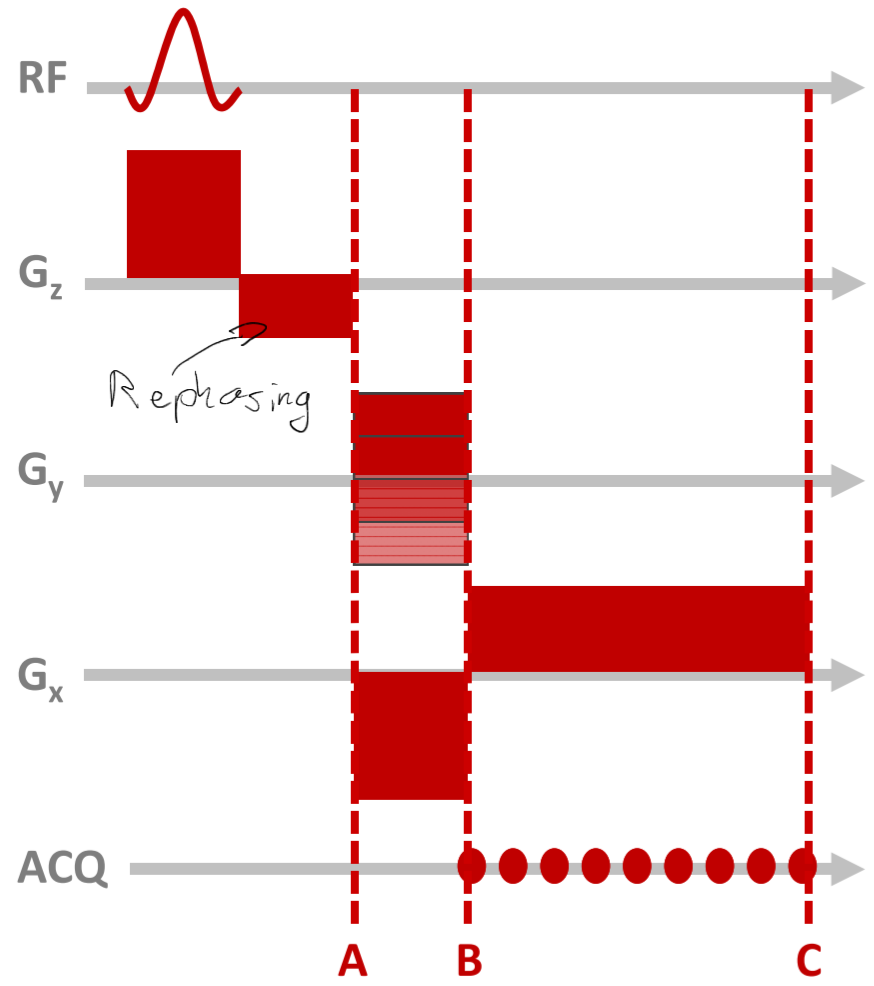
\includegraphics[width = .9\linewidth]{MRI_GradientEcho}
\end{minipage}\\
\textbf{Spin-echo method}: \fbox{$\exp(-t/T_2)$} $T_2^*$ decay (\textbf{const. loc. inhomog.}). $\circlearrowright$ at $T_E/2$ by 180°. $T_E \uparrow$ $\implies$ $T_2$ weight.

Saturation Method \quad $|$ Spin Echo Method\\
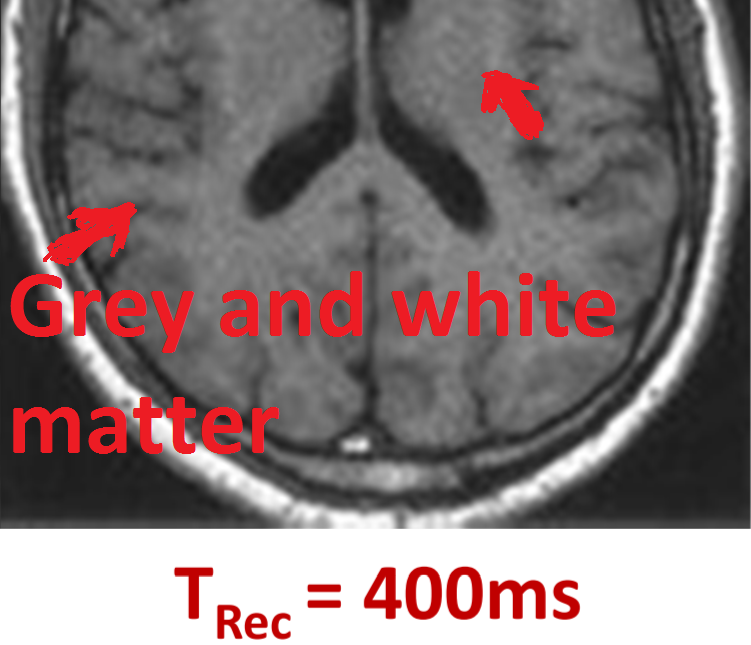
\includegraphics[width = 0.2\linewidth]{MRI_SatMethodShort}
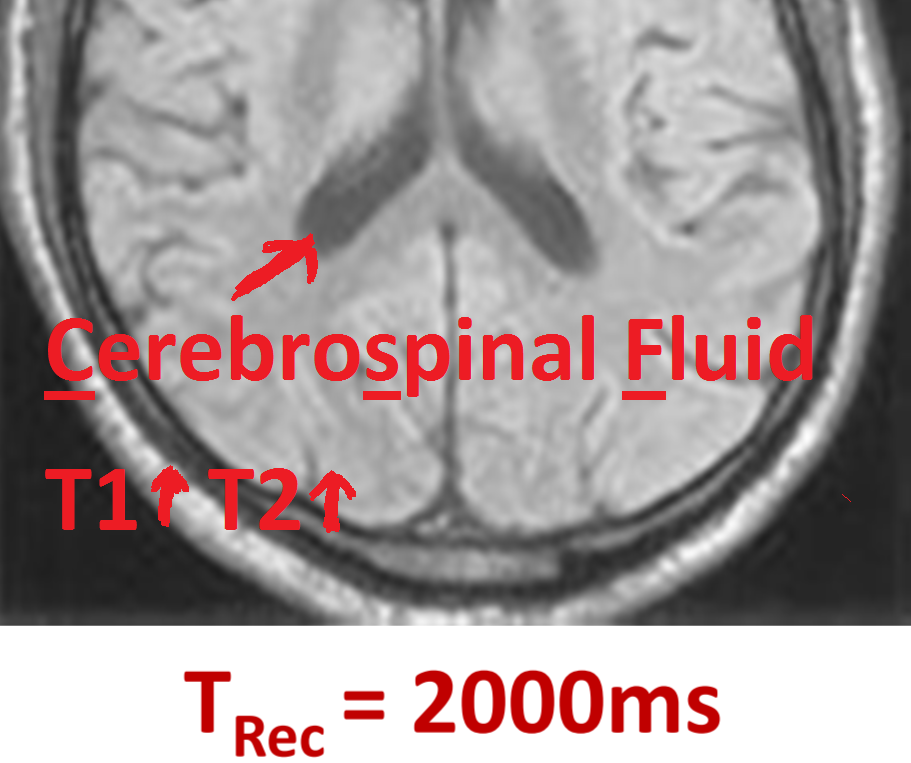
\includegraphics[width = 0.2\linewidth]{MRI_SatMethodLong}
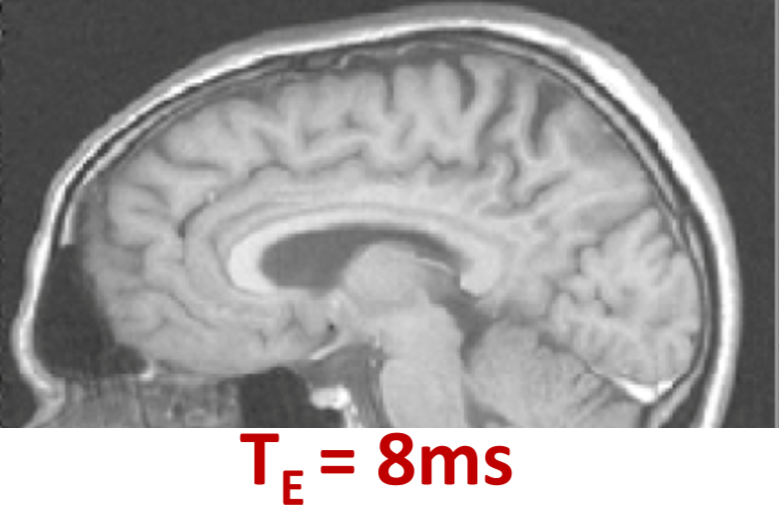
\includegraphics[width = 0.25\linewidth]{MRI_SpinEchoShort}
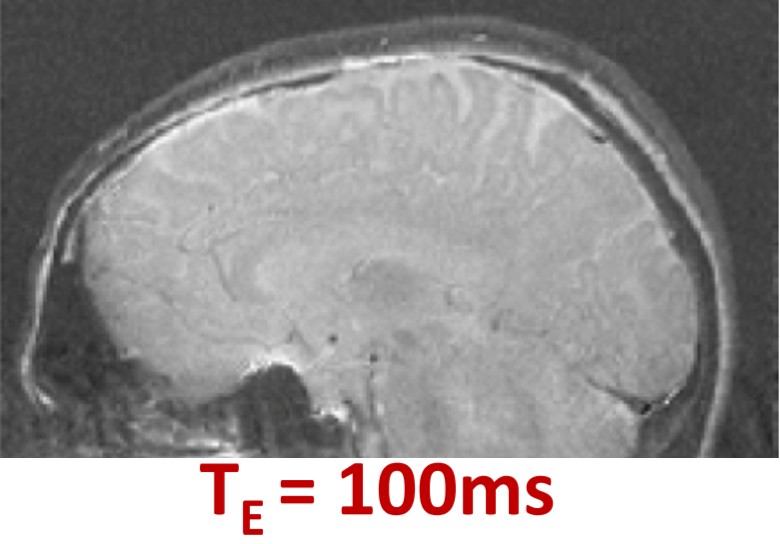
\includegraphics[width = 0.24\linewidth]{MRI_SpinEchoLong}

\textbf{Inflow contrast}: $T_1$ weight. (Blood with $\uparrow M_z$ during $T_R$)
%%%%%%%%%%%%%%%%%%%%%%%%%%%%%%%%%%%%%%%%%%%%%%%%%%%%%%
\subsection{Noise, SNR and Resolution}
$\sigma^2\ped{noise} = 4 k_B \cdot T \cdot R \cdot BW$ \hfill $T$: Temp., $R=U/I$, $BW$: Bandwidth

If frequency indep. and uniform $T$ ($I_0$ is transmit c.):\\
$\highlight{\sigma^2_{noise} = 4 k_B \cdot T \cdot BW \int \sigma(\vec{r}) \frac{\abs{\vec{E}(\vec{r})}^2}{I_0^2}dV}$

Otherwise: $\sigma^2\ped{noise} = 4 k_B \iint T(\vec{r}) \sigma(\omega, \vec{r}) \frac{\abs{\vec{E}(\omega, \vec{r})}^2}{I_0^2} \frac{d\omega}{2\pi} dV$

\fbox{$\sigma^2\ped{noise} = 4 k\ped{B} \cdot BW (R\ap{eff}\ped{sample} T\ped{sample} + R\ap{eff}\ped{coil} T\ped{coil} + R\ap{eff}\ped{env} T\ped{env})$} (last Term usually negligable)

\fbox{$\textbf{SNR} = \frac{\omega B_1^{(-)} (\vec{r}) M_{xy}(\vec{r}) \Delta V}{\sqrt{4 k_B BW (T_{sample}R_{sample} + T_{coil}R_{coil})}} \sqrt{N_{avg}}$}

$BW \propto \text{Gradient strength} \quad \propto \text{Body size} \quad \propto t\ped{acq}^{-1}$\\
$\quad t_{scan} \propto N_{avg} \quad \implies \highlight{SNR \propto \Delta V \sqrt{t}}$

SNR$\uparrow$: magnetization$\uparrow$ by $B_0\uparrow$. $\omega\uparrow$. $T\ped{coil}\downarrow$, $R\ped{coil}\downarrow$

\textbf{Resolution limits}:\\
In k-space, the image is multiplied with\\
$H(k) = \textrm{rect}\left( \frac{k}{2 k\ped{max}}\right) \eu^{-t/T_2^*} \quad \implies \textbf{PSF}:\: \highlight{\Delta x \geq \frac{\pi}{\gamma G\ped{max} T_2^*}}$\\

Diffusion Area: $\left< \Delta x^2 \right> = 6 \cdot D \cdot T\ped{acq}$ \hfill $D = \unitfrac[10^{-3}]{mm^2}{s}$ for $\ce{H_2O}$.
%%%%%%%%%%%%%%%%%%%%%%%%%%%%%%%%%%%%%%%%%%%%%%%%%%%%%%
\subsection{Various}
\textbf{T/R Switch}: Block kW in transmit mode, nW in r mode.

\textbf{RF Body Coil - Gradients - $B_0$-Magnet (3-7T) - Shield Coils - Cryogenics} @4K.

\fbox{$\unit[1]{Gauss} = \unit[0.1]{mT}$} \textbf{Limits}: 5 Gauss: Pacemakers, Credit cards. --- 50 Gauss magnetic objects

\subsubsection{fMRI \textnormal{-- functional MRI (brain imaging)}}
Oxygenated hemoglobin is diamagnetic, deoxy-Hb is paramagnetic. Param. disturbs the B-field $\implies$ reduces $T_2^*$. $S_{task} > S_{idle}$. Use echo planar imaging because it is fast.\\
Calc \textbf{scalar product} of activation and \textbf{paradigm} ($\pm 1$)

		%! Author = tstreule

\section{Ultrasound Imaging \textnormal{\normalsize $c\ped{sound} \simeq \unitfrac[1540]{m}{s}$}}

Frequencies of 1-50 MHz $\implies$ $\lambda = 1 .... 0.03 \unit{mm}$

Wave formula: $\nabla^2 p - \frac{1}{c^2} \frac{\partial^2 p}{\partial t^2} = 0$ \quad Max. p = compressional pressure= $p_c$, \quad Min. p = rarefactional pressure = $p_r$

$\kappa$ = compressibility, $\rho$ = density, $u_z$ = particle velocity\\
$c = \frac{1}{\sqrt{\kappa \rho}}$, \quad $p = \rho c u_z$, \quad $Z = p/u_z = \rho c = \sqrt{\frac{\rho}{\kappa}}$, \quad $I = p u_z / 2$

Pressure \textbf{coeff.}: \highlight{$\displaystyle r = \frac{Z_2 - Z_1}{Z_2 + Z_1}$} \highlight{$\displaystyle t = \frac{2Z_2}{Z_2 + Z_1}$}\\
\textbf{Refraction:} $\theta_i = \theta_r$, \quad $\sin\theta_i/\sin\theta_t = c_i/c_t$

\textbf{Rayleigh scattering} by structures smaller $\lambda$ $\to$ speckles/noise ($\sigma_S \propto \lambda^{-4}$). It has a char. length of $\lambda/2$:

\textbf{Attenuation} (due to scattering and absorption): \\
\highlight{$\displaystyle p(z) = p_0 e^{-\alpha z} \approx p_0\,10^{-\frac{\textrm{att}}{\unit[20]{dB} }}$} ($[z]=\unit{cm}$, $\textrm{att} = \alpha_0\cdot z = \textrm{const}\cdot f\cdot z$) \\
\textbf{Decibel notation}: $\alpha_0 = 20 \log \left( \frac{p_0}{p(z)} \right) \frac{1}{z} = 8.686 \alpha [dB/cm]$

\textbf{Transducer}: Tx/Rx switch, Damping, matching layer, $f_0$
%%%%%%%%%%%%%%%%%%%%%%%%%%%%%%%%%%%%%%%%%%%%%%%%%%%%%%
\subsection{Beam geometry}
%
\textbf{Near field (Fresnel)}zone with const. beamwidth of $2r$.\\
\textbf{Far field (Fraunhofer)} zone which starts at \highlight{$\displaystyle \textrm{NFB} \approx \frac{r^2}{\lambda_{tissue}}$}.\vspace{-3mm}\\
Beamwidth = lateral resolution \vspace{1mm}

\textbf{Angle} of beam: \highlight{$\displaystyle \theta = 2\arcsin\left( \frac{0.61 \lambda}{r}\right)$}

\textbf{Focusing} with acoustic lens: Focal distance, lateral resolution, aperture dimension. Depth of focus: Over which distance is it narrow.\vspace{-1mm} \\
\textbf{Axial resolution}: \highlight{$\textstyle \Delta z \geq \frac{\lambda}{2} = \frac{p_dc\ped{sound}}{2}$} \quad $\lambda$: pulse length

\textcolor{gray}{ \textbf{Range Gain}: The longer signals take to come back, the $\downarrow$. To compensate: Amplify the late signals exponentially }

\textbf{Thermal noise}: \fbox{$P_N = k_B \cdot T \cdot BW [\unit{W}]$} \hfill (BW: typ. 1MHz)

\textbf{SNR in dB} = Transmitted Power - power losses - $P_N$.\\
Power losses: Attenuation \& reflection coefficient (factor 20)
%%%%%%%%%%%%%%%%%%%%%%%%%%%%%%%%%%%%%%%%%%%%%%%%%%%%%%
\subsection{Transducer setups}
%
\textbf{Linear Array}. \textbf{pitch} $d \approx \lambda$ and \textbf{kerf} (gap). Sweep through. Good resolution $\implies$ small pitch $\implies$ large $\theta$

\begin{minipage}{0.64\linewidth}
    \textbf{Phased parallel operation}:\\
    \highlight{$\displaystyle \Delta \Phi = k \Delta s = kd\sin\alpha \mod 2\pi$}. Multiple solutions for \fbox{$d > \lambda/2$ $\to$} \textbf{grating lobes} (weaker since not time aligned)
\end{minipage} \hfill
\begin{minipage}{0.35\linewidth}
    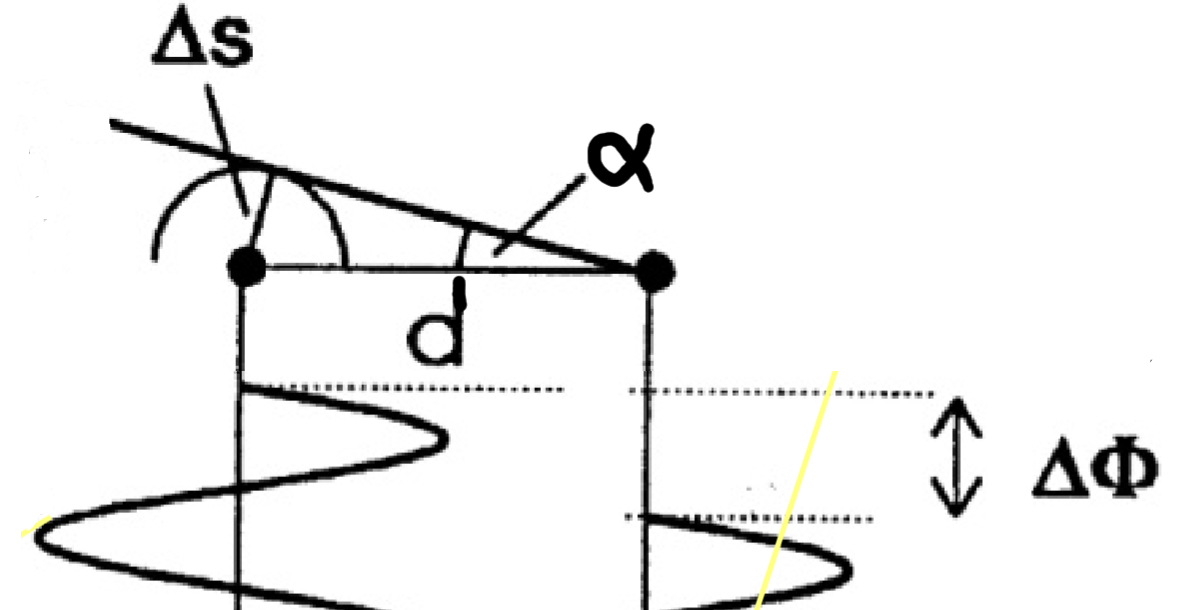
\includegraphics[width=\linewidth]{US_PhasedParallelMode}
\end{minipage}

Receiving analog: delay elements, then sum all up.

\textbf{Variable focusing} (with shifting) and a combination of all

\textbf{Multi-dim. arrays}: 2D or 1.5D ($1/2$ D = ``\textbf{elevation}'').

\textbf{Curved arrays} (instead of flat): For small acoustic windows

\textbf{Annular Array} (circular sections): Simpler adjustable focus and circular symmetry = more \textbf{isotropic depiction}
%%%%%%%%%%%%%%%%%%%%%%%%%%%%%%%%%%%%%%%%%%%%%%%%%%%%%%
\subsection{Scanning modes}
%
\textbf{A-Mode} (Amplitude): time (distance) vs amplitude. \\
Usage: e.g. measuring the thickness

\textbf{M-Mode} (Motion): time vs depth. Amplitude with brightness. Must be tilted manually

\textbf{B-Mode} (Brightness): 2D spacial. Amplitude with brightness

\textbf{Scanning Procedures}:\\
$\bullet$ \textbf{Parallel scan} for large acoustic window.
$\bullet$ \textbf{Sector scan} for small ac. window.
$\bullet$ \textbf{Radial scan} for transd. in blood vessels (measuring the vessel wall).
$\bullet$ \textbf{Compound scan} from different directions $\to$ redundancy and reduce speckles.
%%%%%%%%%%%%%%%%%%%%%%%%%%%%%%%%%%%%%%%%%%%%%%%%%%%%%%
\subsection{Measuring the blood flow}
%
Observer at velocity $v$, receives $f\ap{eff} = f \frac{c + v}{c}$

Blood vessel flows under the receiver with angle $\theta$ rel. to the vertical to transducer:
\fbox{$f\ped{rec} = f_i \frac{2 f_i \cos \theta}{c} + \frac{f_i v^2 \cos^2 \theta}{c^2}$}\\
\begin{minipage}{0.6\linewidth}
    \highlight{$\displaystyle f_D = f_i - f\ped{rec} \approx \frac{2 f_i v \cos \theta}{c}$}
\end{minipage}
\begin{minipage}{0.4\linewidth}
    Must know $\theta$ \\$\implies$ do B-Mode scan first
\end{minipage}

Red blood cells $\approx 7 \unit{\mu m}$ wide $\implies$ Use high freq., typ. 5MHz

\textbf{Cont. setup}: Separated receiver/transmitter. Quadr. encoder: Mult. with cos ($\to$ real part) and sin ($\to$ imag part) $\to$ double sided spectrum. Neg. side is \textit{negative flow}. Then \textit{low-pass + high-pass} to remove (quasi) stationary echos.

\textbf{Pulsed measurement}: 1 transducer. Only receive signal during a narrow time window. Its delay = depth.

\begin{minipage}{\linewidth}
    \raggedleft
    \vspace{2mm}
    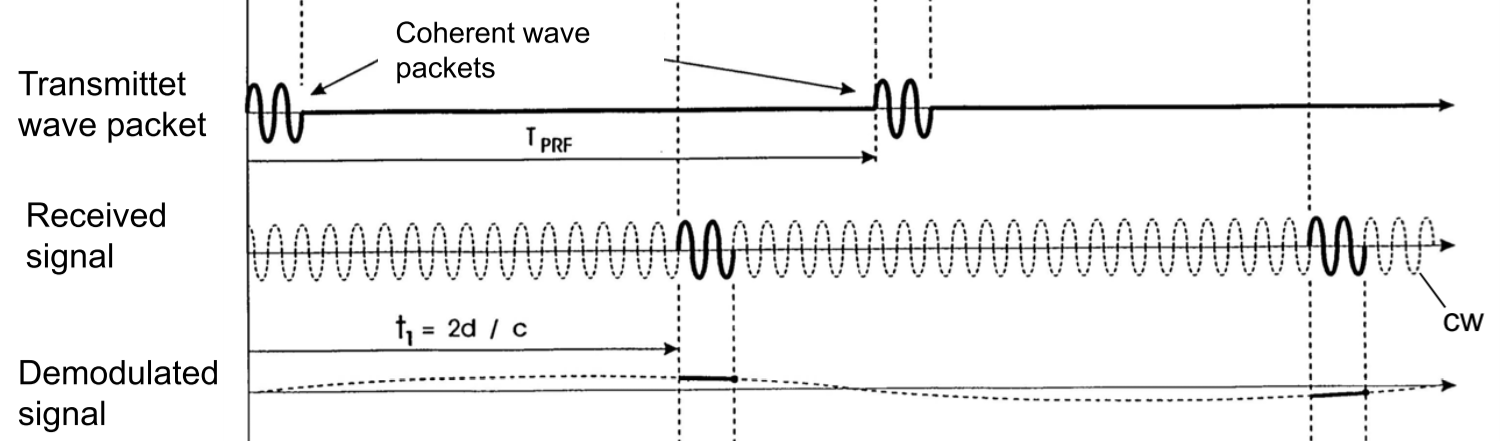
\includegraphics[width = \linewidth]{US_DopplerPulsed} \vspace{-37mm}\\
    \highlight{$\displaystyle -f\ped{prf}/2 < f\ped{D} < f\ped{prf}/2$}
    \vspace{37mm}
\end{minipage}
%%%%%%%%%%%%%%%%%%%%%%%%%%%%%%%%%%%%%%%%%%%%%%%%%%%%%%
\subsection{Appendix}
%
\begin{tabular}{ c@{$\;\laplace\;$}c c c@{$\;\laplace\;$}c }
    $f(at)$			& $\frac{1}{\abs{a}}F(s/a)$	&& $f(t-a)$		& $\eu^{-as}F(s)$\\
    $f(t)\eu^{at}$	& $F(s-a)$					&& $f'(t)$		& $sF(s) - f(0^+)$\\
    $t^n$			& $n!/s^{n+1}$				&& $t^n f(t)$	& $(-1)^n F^{(n)}(s)$\\
    $\sin(at)$		& $\frac{a}{s^2 + a^2}$		&& $\cos(at)$	& $\frac{s}{s^2 + a^2}$\\
    $\eu^{at}$		& $\frac{1}{s - a}$			&& $t^n \eu^{at}$& $\frac{n!}{(s-a)^{n+1}}$
\end{tabular}

\textbf{Constants}:\\
\begin{tabular}{r@{$\;=\;$}l}
    $h$			& $\unit[6.626\E{-34}]{JS} = \unit[4.135\E{-15}]{eV\,s}$,\qquad $\hbar = \frac{h}{2\pi}$\\
    $\epsilon_0$& $\unitfrac[8.85\E{-5}]{As}{Vm}$\\
    $\mu_0$		& $\unitfrac[4\pi\E{-7}]{N}{A^2}$\\
    $k\ped{B}$	& $\unitfrac[1.38\E{-23}]{J}{K} = \unitfrac[8.617\E{-5}]{eV}{K}$\\
    $q$			& $\unit[1.602\E{-19}]{C}$, \quad $m_e = \unit[9.109\E{-31}]{kg}$, \quad $m_p = \unit[1.672\E{-27}]{kg}$\\
    $m_ec^2$	& $\unit[511]{eV}$
\end{tabular}
$\unit[0]{^\circ C} = \unit[273.15]{K}$


	\end{multicols*}
\end{document}
